\documentclass[11pt]{myclass}

\usepackage{amssymb,amsmath,amsfonts,pdfpages,color, url}
\usepackage{booktabs}
\usepackage{wrapfig}
\usepackage{amsmath}
\usepackage{multirow}

\newtheorem{cor}[theorem]{Corollary}
\newtheorem{rem}{Remark}[section]
\newtheorem{addendum}[theorem]{Addendum}
\newtheorem{definition}[theorem]{Definition}
\newtheorem{exa}{Example}[section]
\newtheorem{Notation}[theorem]{Notation}
\newtheorem{question}[theorem]{Question}
\newtheorem{convention}[theorem]{Convention}
\newtheorem{Assumption}[theorem]{Assumption}
\newcommand{\R}{\ensuremath{\mathbb{R}}}

\def\dis{\mathop{\displaystyle}}
\def\Train{\mathop{\rm Train}}
\def\Test{\mathop{\rm Test}}
\newcommand{\bb}{\ensuremath{{\rm{\bf b}}}}
\newcommand{\w}{\ensuremath{{\rm{\bf w}}}}
\def\Gsim{\mathop{\Gamma}}

%%% ----------------------------------------------------------------------


\begin{document}


\title{Project Final Report \\ Title: Inferring transportation modes from GPS trajectories}

\author{Sole Team Member: Hasan Pourmahmoodaghababa \\
\texttt{uID: u1255635}}


\maketitle


\begin{abstract}
In this project, using a conditional Markov model (CMM), also called maximum entropy Markov model (MEMM) and recurrent neural networks (RNN, specially LSTM) we try to infer transportation modes from GPS trajectories. We employ the feature mapping defined in \cite{PT19a}, length, velocity and acceleration of trajectories to infer transportation modes. We show that CMM outperforms other inferring methods available in the literature that the author is aware of. 
\end{abstract}


\section{Introduction}

Transportation modes analysis is one of the hot research areas in transportation and traffic research area. In fact, travel mode choice is a typical behavior attribute of people and so is of interest for researchers. Nowadays with the advent of Global Positioning System (GPS), it is easy to collect travel data, for instance through mobile phones, in contrast with the old days where people had to obtain data through a survey for example. This has led to more interest in research in this area and absorbed many researchers. 

Understanding mobility patterns in mining GPS datasets has many applications like learning significant locations and identification of transportation modes (see \cite{LH2014, LS2020, DH2018, DCHR2020} and references therein). Authors in \cite{DH2018, DCHR2020, ETNK2016, WLJL2017} utilize convolutional neural networks to infer transportation modes and a hidden Markov model is employed in \cite{LS2020} for this purpose. All these papers focus on Geolife dataset (see Subsection \ref{dataset}) which we also would like to analyze it here. 

In this project we will apply two models with several feature mappings. The first model is a {\it conditional Markov model} (CMM) also called {\it maximum entropy Markov model} (MEMM), which is a next-state model. In this model we will use some machine learning classical classifiers such as SVM, Decision tree and Random Forest as local models to get local scores for each state. Then for inference step we will apply Viterbi algorithm. The next model is a {\it recurrent neural network} (RNN), which is appropriate for sequential data analysis. Indeed, for we will leverage the special RNN termed {\it long-short-term-memory} (LSTM) where the previous states' information is transferred as a memory to the next state and so preserves the global dependencies in data, and hence suitable for structured predictions. 

%All the supplementary materials are included in the GitHub repository 

%\url{https://github.com/aghababa/Transportation-Modes-Stuctured-Prediction}. 

\section{Definitions and Feature Mappings}

In this section we give some definitions and introduce the feature mappings we will use in this project. 

\paragraph{Curve.}
By a {\it curve} we mean the image of a continuous map $\gamma: [0,1] \to \mathbb{R}^2$. The set of curves is denoted by $\Gamma$. 

So, note that we are only considering the geometric shape of curves and so two different maps can have a same curve. For instance, if $\gamma$ is a curve, then $\gamma$ and $\overline{\gamma}$, where $\overline{\gamma}(t) = \gamma(1-t)$, are considered the same curves as they are the same geometrically. However, their direction is not the same and thus they are not the same as two maps. 

\paragraph{Trajectory.}
By a {\it trajectory} we mean a finite sequence of triples $(a, b, t)$, where $a$ and $b$ denote latitude and longitude of a moving object and $t$ is the timestamp showing the time where the object was at $(a, b)$ position in $x, y$-coordinate at that time. Assuming $\{(a_i, b_i, t_i) : 0 \leq i \leq m\}$ is a trajectory, connecting consecutive $(a_i, b_i)$'s by a line segment we get a piece-wise linear curve, which we call it trajectory as well. Therefore, the set of trajectories is a subset of $\Gamma$. 

\paragraph{Feature Mapping.} \label{features}
Let $\gamma \in \Gamma$ be a curve and let $q \in \mathbb{R}^2$ be a landmark. According to \cite{PT19a} we define $v_q: \Gamma \to [0, \infty)$ by 
\[
v_q(\gamma) = {\rm dist}(q, \gamma) = \min_{p \in \gamma} \|q-p\|,
\]
where $\|\cdot\|$ is the $l^2$-norm on $\mathbb{R}^2$. Now let $Q = \{q_1, q_2, \ldots, q_n\} \subseteq \mathbb{R}^2$ be a set of landmarks. Then, as it is introduced in \cite{PT19a}, we can define a feature mapping $v_Q: \Gamma \to \mathbb{R}^n$ by 
\[
v_Q(\gamma) = (v_{q_1}(\gamma), v_{q_2}(\gamma), \ldots, v_{q_n}(\gamma)).
\]
This also give a distance on $\Gamma$ provided that $Q$ is sufficiently dense in a bounded region containing all curves under consideration \cite{PT19a}. The distance is given by $d_Q(\gamma_1, \gamma_2) = \|v_Q(\gamma_1) - v_Q(\gamma_2)\|$.

It is worth noting that it is commented that in practice 20 landmarks are usually enough for trajectory data analysis tasks. 

We will use a trajectory dataset and so we can define three more features, namely {\it average length}, {\it velocity} and {\it acceleration}. More formally, for a trajectory $\gamma = \{(a_0, b_0, t_0), \ldots, (a_m, b_m, t_m)\}$ we consider 
\[
\displaystyle \text{length} = \frac{1}{m} \sum_{j=1}^m \|(a_j, b_j) - (a_{j-1}, b_{j-1})\|,
\]
\[\text{velocity}= \frac{1}{m} \sum_{j=1}^m \frac{\|(a_j, b_j) - (a_{j-1}, b_{j-1})\|}{t_j},\]
\[\text{acceleration} = \frac{1}{m} \sum_{j=1}^m \frac{\|(a_j, b_j) - (a_{j-1}, b_{j-1})\|}{t_j^2}.\]
Using these features, we can have a bunch of feature mappings:
\begin{itemize}
\item[1)] $\phi_1(\gamma) = (\text{length}, \text{velocity}, \text{acceleration}) \in \mathbb{R}^4$;

\item[2)] $\phi_2(\gamma) = (a_0, b_0, a_m, b_m, \text{length}, \text{velocity}, \text{acceleration}) \in \mathbb{R}^{8}$;

\item[3)] $\phi_3(\gamma) = v_Q(\gamma) \in \mathbb{R}^{|Q|}$;

\item[4)] $\phi_4(\gamma) = (v_Q(\gamma), \text{length}, \text{velocity}, \text{acceleration}) \in \mathbb{R}^{|Q|+4}$;

\item[5)] $\phi_5(\gamma) = (v_Q(\gamma), a_0, b_0, a_m, b_m, \text{length}, \text{velocity}, \text{acceleration}) \in \mathbb{R}^{|Q|+8}$;
\end{itemize}



\section{Experiments} \label{experiments}

In this section we run some experiments to examine our selected models' performance. 

\subsection{Data} \label{dataset}
The dataset we employ here is Geolife GPS Trajectory dataset \cite{geolife-gps-trajectory-dataset-user-guide}, available for public\footnote{\url{https://msropendata.com/datasets/d19b353b-7483-4db7-a828-b130f6d1f035}}, which is released by Microsoft. It consists of trajectories of 182 users from 2007 to 2012. The dataset consists of 17,621 trajectories which are mostly recorded in Bejing, China. To have a pictorial sense of data, see Figure \ref{data}, where one is taken from the user guide of the data and the other is generated by the author.  

\begin{figure}[h]
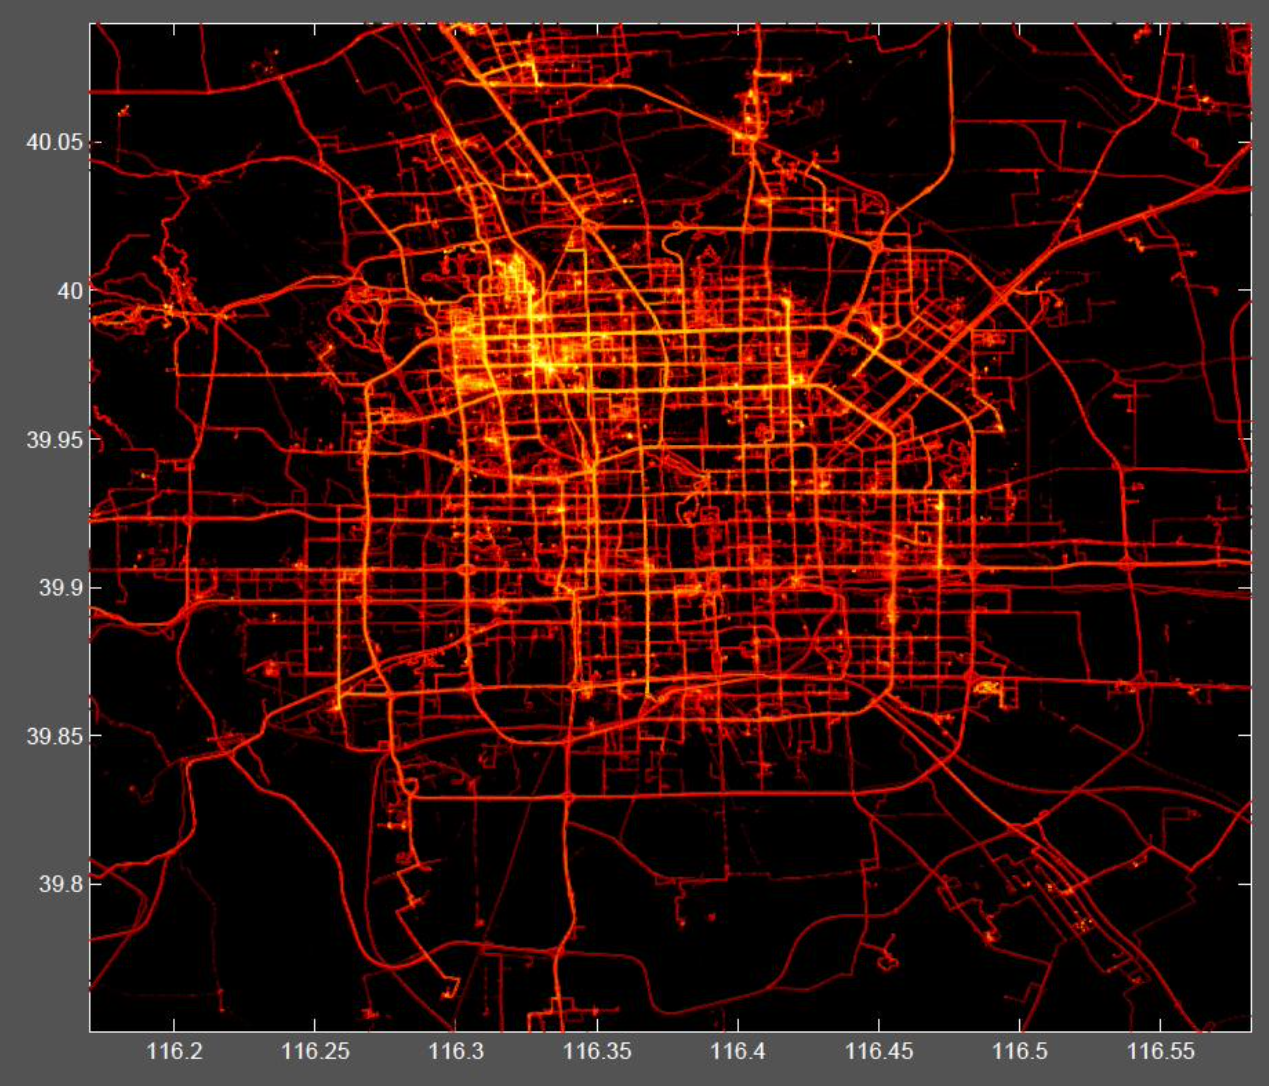
\includegraphics[width=0.5 \textwidth]{data1}
\hfill
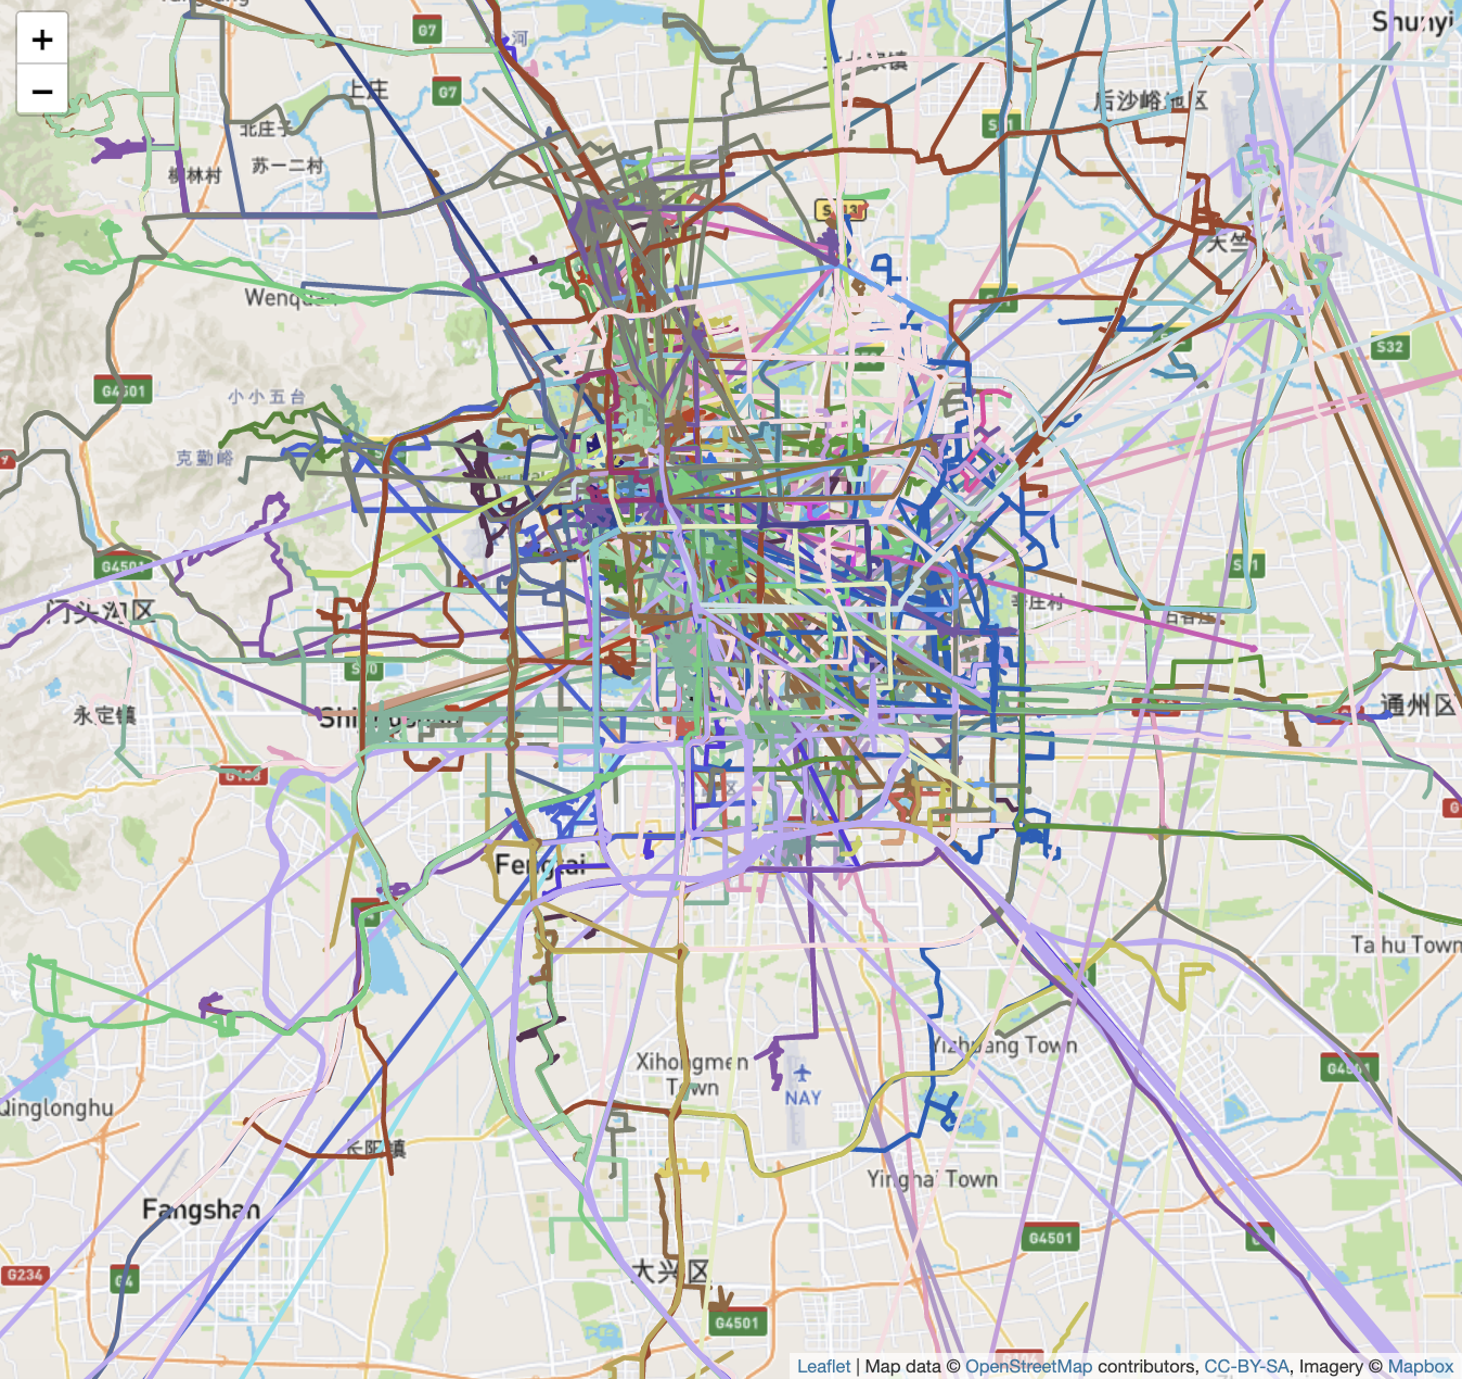
\includegraphics[width=0.451 \textwidth]{Geolife} 
\caption{Left: Distribution of the dataset in Beijing city (taken from the user guide of the data). Right: Visualizing Geolife GPS Trajectory Dataset on the map (about 18,000 trajectories, created by the author).}
\label{data}
\end{figure}

Among 182 users 69 of them have labeled their trajectories with transportation modes such as walk, bike, bus, car, taxi, subway, railway, train, airplane, motorcycle, run. As other modes are in extreme minority in the labeled data, we will only consider walk, bike, bus, car, taxi, subway, railway and train. Moreover, as it is recommended in the user guide of data, we regard car and taxi as one transportation mode, namely car, and similarly, we regard all three labels train, railway and subway as train. Therefore, we end up with 5 labels (walk, bike, bus, car and train). 

\subsection{Preprocessing} 

First we remove trajectories without a label as well as each part of a trajectory having no matchable label. Then we partition each labeled GPS trajectory of each user into some sub-trajectories (trips) according to the time interval. In fact, for partitioning, we use the threshold 20 minutes recommended in \cite{ZLWX} and is applied in several studies like \cite{DH2018, DCHR2020}. In this way, we obtain about 10,000 trajectories with only 1 label, 1,700 trajectories with 2 labels and less than 100 trajectories with 3 or 4 labels. Considering a trajectory as a sequence of trips (remember that each trip consists of only one label), we get 10,000 sequences of length 1, 1,700 sequences of length 2 and less than 100 sequences of length 3 or 4. However, we need more sequences with longer lengths. Thus we decided to generate more sequences with lengths 3, 4 and 5. We do this utilizing 10,000 sequences of length 1, by randomly concatenating some of them together. At the end, we get about 5,400 trajectories such that lengths (belonging to $\{1,2,3,4,5\}$) are evenly distributed. 

We remark that generating sequence elements by random will possibly not enforce an essential structure on previous states of the sequence. This means that if we have a real data having such sequences, the performance of our models will definitely be better than what we will get here. 

\subsection{Experimental Setup}
We can consider our problem as a part-of-speach tagging problem, where we would like to assign our 5 labels to these 5,000 trajectories. The first model we use is CMM and the next one is LSTM. In both models, the preprocessed data is randomly split to train and test datasets by 2/3 of data as train data and 1/3 as test data. 

\subsubsection{Conditional Markov Model} 
To use CMM, we apply 5 feature mappings associated with $\phi_i$ in Section \ref{features}. Indeed, let $x = (x_1, x_2, \ldots, x_n)$ be a trajectory with label $y = (y_1, y_2, \ldots, y_n) \in \{0,1,2,3,4\}^n$ ($1\leq n \leq 5$), where each $x_i$ is a sub-trajectory having label $y_i$. Then for each $j \in \{1,2,3,4,5\}$, using the next-state model $p(y_i | y_{i-1}, \phi(x_i))$, we define 
\[
\Phi_j(x_0) = \phi_j(x_0), \quad \Phi_j(x_i, y_{i-1}) = (\phi_j(x_i), y_{i-1}), 
\] 
and so, $\Phi_j(x, y) = (\Phi_j(x_0), \Phi_j(x_1, y_0), \ldots, \Phi_j(x_n, y_{n-1}))$. 

Applying these feature mappings, we use 4 ML classifiers Linear SVM, Gaussian SVM, Decision Tree and Random Forest as local scoring functions. Last but not least is inferring step which we employ the {\bf Viterbi} algorithm which is implemented by the author from scratch. Accuracy results are given in Table \ref{table-CMM}. As it can be seen, the conditional Markov model with feature mapping $\Phi_4$ and Random Forest as a local classifier outperforms others and we get $83.2\%$ test accuracy.  


\begin{table}[htbp]
\centering
\begin{tabular}{|c|l|c|c|}
\hline
       {\bf Feature Mapping} &  {\bf Local Classifier}  &   {\bf Train Accuracy} &  {\bf Test Accuracy}   \\
\hline 
\multirow{4}{*}{\rotatebox[origin=c]{0}{$\Phi_1$}}  
	& Linear SVM, $C=1$  &      0.5111 &    0.5043  \\ 
	& Gaussian SVM, $C = 1e5$, $\gamma = 10$   &   0.5729  &  0.4820   \\
        & Decision Tree &      1.0000 &        0.6744   \\
        &  Random Forest with 100 estimators &      0.9918 &     {\bf 0.7310}   \\
\hline 
\multirow{4}{*}{\rotatebox[origin=c]{0}{$\Phi_2$}}  
	& Linear SVM, $C=0.01$  &      0.5162 &    0.5102  \\ 
	& Gaussian SVM, $C = 1e4$, $\gamma = 0.1$   &   0.6226  &  0.5475   \\
         & Decision Tree &      1.0000 &        0.7374   \\
         & Random Forest with 100 estimators &      1.0000&     {\bf 0.8208}   \\
\hline 
\multirow{4}{*}{\rotatebox[origin=c]{0}{$\Phi_3$}}  
	& Linear SVM, $C=1e8$  &      0.4276 &    0.4290  \\ 
	& Gaussian SVM, $C = 1e4$, $\gamma = 1$   &   0.5467  &  0.4882   \\
         & Decision Tree &      1.0000 &        0.6825   \\
         & Random Forest with 100 estimators &      1.0000 &     {\bf 0.7294}   \\
\hline 
\multirow{4}{*}{\rotatebox[origin=c]{0}{\color{blue} $\bf \Phi_4$}}  
	& Linear SVM, $C=1$  &      0.5218 &    0.5282  \\ 
	& Gaussian SVM, $C = 1e4$, $\gamma = 1$   &   0.7336  &  0.5287   \\
         & Decision Tree &      1.0000 &        0.7343   \\
         & Random Forest with 100 estimators &      0.9999 &     {\color{blue} \bf 0.8316}   \\
\hline 
\multirow{4}{*}{\rotatebox[origin=c]{0}{$\Phi_5$}}  
	& Linear SVM, $C=1$ &      0.5279 &    0.5144  \\ 
	& Gaussian SVM, $C = 1e4$, $\gamma = 1$   &   0.7554  &  0.5252   \\
         & Decision Tree &      1.0000 &        0.7452   \\
         & Random Forest with 100 estimators &      1.0000 &     {\bf 0.8276}   \\
\hline 
\end{tabular}
\caption{CMM-based transportation modes' train and test accuracies (66/33 train/test split) for Beijing dataset using 5 feature mappings. Notice 20 landmarks are chosen randomly around curves to get the feature mappings $\Phi_3, \Phi_4, \Phi_5$.}
\label{table-CMM}
\normalsize
\end{table}


\subsubsection{Recurrent Neural Networks}

In this experiment we apply LSTM to predict transportation modes of GPS trajectories. We apply above five feature mappings with two different LSTM architectures and 66/33 train-test split. These neural networks are implemented in pytorch on a 16 GB Ram and 2 GHz Quad-Core Intel Core i5 system. 

\paragraph{First Architecture.} 
The first one is a simple 1-layer LSTM with 1 fully connected layer neural network. The negative log likelihood function (torch.nn.NLLLoss()) is chosen as loss function. We also tried with cross entropy loss (torch.nn.CrossEntropyLoss()) and got roughly the same results. Different number of hidden layers and learning rates are applied to tune hyperparameters and get a robust and high performance model. Train and test accuracies are presented in Table \ref{table-LSTM1}. As it can be viewed, the feature mapping $\Phi_4$ outperforms others with $64.3\%$ test accuracy. 

\begin{table}[htbp]
\centering
\begin{tabular}{|c|c|c|c|c|}
\hline
       {\bf Feature Mapping} &  {\bf Hidden Dimension} &  {\bf Learning rate}  &   {\bf Train Accuracy} &  {\bf Test Accuracy}   \\
\hline 

$\Phi_1$	& 20  &  0.005 &   0.6310 &    0.6294  \\ 
\hline 
$\Phi_2$	& 200  &   0.0008 &   0.6001 &    0.6022  \\ 
\hline 
$\Phi_3$	& 100 &   0.001 &   0.3732 &    0.3733  \\ 
\hline 
{$\bf \Phi_4$}	& 20  &   0.01 &   0.63.34 &   {\bf 0.6427}  \\ 
\hline 
$\Phi_5$	& 200 &   0.001 &   0.6329 &    0.6357  \\ 
\hline 
\end{tabular}
\caption{Transportation modes' train and test accuracies for Beijing dataset based on LSTM with 1 fully connected layer, using 5 feature mappings. 20 landmarks are chosen randomly around curves to get the feature mappings $\Phi_3, \Phi_4, \Phi_5$.}
\label{table-LSTM1}
\normalsize
\end{table}

\paragraph{Second Architecture.} 
The next one is a multi-layer LSTM with 2 fully connected layers neural network. The loss function is again negative log likelihood function. We tried this architecture with more LSTM layers but we found the more layers the less test accuracies. Therefore, we used only 1 layer of LSTM. Different number of hidden layers and learning rates are applied to tune hyperparameters and get a robust and high performance model. In this architecture, similarly, we can observe that the feature mapping $\Phi_4$ outperforms others with $65\%$ test accuracy.

\begin{table}[htbp]
\centering
\begin{tabular}{|c|c|c|c|c|c|}
\hline
       {\bf Feature Mapping} &  {$\rm \bf Hid\_dim\_1$} &  {$\rm \bf Hid\_dim\_2$} &  {\bf Learning rate}  &   {\bf Train Accuracy} &  {\bf Test Accuracy}   \\
\hline 

$\Phi_1$	& 10  & 20  &  0.02 &   0.6382 &    0.6276  \\ 
\hline 
$\Phi_2$	& 100  & 200  &  0.005 &   0.5089 &    0.5223  \\ 
\hline 
$\Phi_3$	& 20 &  20  & 0.01 &   0.3676 &    0.3753  \\ 
\hline 
$\bf \Phi_4$	& 100  & 50  &  0.001 &   0.6560 &    {\bf 0.6495}  \\ 
\hline 
$\Phi_5$	& 200 &  100  & 0.0015 &   0.6085 &    0.5966  \\ 
\hline 
\end{tabular}
\caption{Transportation modes' train and test accuracies for Beijing dataset based on LSTM with 2 fully connected layers, using 5 feature mappings. 20 landmarks are chosen randomly around curves.}
\label{table-LSTM2}
\normalsize
\end{table}


\subsection{Baseline Case}

As a baseline approach, we try to predict transportation modes of trajectories independent from each other, i.e., considering the problem as a multi-class classification task. We apply K-nearest neighbor search (KNN), Gaussian kernel SVM, Decision Tree and Random Forest with feature mappings $\phi_i$ ($1 \leq i \leq 5$). Nevertheless, we have included the best performed feature mapping ($\phi_4$) results. The setup is clear as it is a multi-class classification and we utilize sklearn classifiers with 66/33 train-test split. The chosen hyperparameters and train and test accuracies are included in Table \ref{table-multi-class}. We have done each classification method for 100 times and reported the average train and test accuracies along with their standard deviations. As it can be viewed, Random Forest outperforms other classifiers with $82.3\%$ accuracy. 

\begin{table}[htbp]
\centering
\begin{tabular}{|l|c|c|c|}
\hline
          {\bf Classifier}  &   {\bf Train Accuracy} &  {\bf Test Accuracy} &  {\bf Standard Deviation}  \\
\hline 
	KNN with 5 centers &      0.8117 &        0.7449 &    0.0102  \\ 
	Gaussian kernel SVM, $C = \gamma = 1e4$ &   0.0100  &   0.7274 &  0.0112  \\
         Decision Tree &      1.0000 &        0.7562 &    0.0109  \\
         Random Forest with 100 estimators &      1.0000 &     {\bf 0.8230} &    0.0089  \\
\hline 
\end{tabular}
\caption{Multi-class classification train and test accuracies for Beijing dataset using $\phi_4$ vectorization. 20 landmarks are chosen randomly around curves.}
\label{table-multi-class}
\normalsize
\end{table}


\section{Comparison With Previous Studies}

Although the experimental setup in \cite{DCHR2020} is somehow different and makes comparison a bit hard, our $83.2\%$ test accuracy outperforms the best test accuracy $76.8\%$ reported there. The test accuracy $84.8\%$ reported in \cite{DH2018} is achieved by convolutional neural network with 80/20 train/test split. For the sake of comparison we did our CMM-based experiments with Random Forest as a local classifier and 80/20 train/test split and got $85\%$ accuracy on test data using feature mapping $\Phi_4$ and 50 randomly chosen landmarks; see Table \ref{table-CMM-RF} for train and test accuracies. However, it is worth noting that we could play with some hyperparameters, like the number of estimators or entropy type selection in Random Forest or increasing the number of landmarks or choosing them in an optimal way, to increase the accuracy a bit more. 

\begin{table}[htbp]
\centering
\begin{tabular}{|c|c|c|c|c|c|}
\hline
       {\bf Feature Mapping} &  {\bf Local Classifier} &  {\bf \# Estimators}  &   {\bf Train Accuracy} &  {\bf Test Accuracy}   \\
\hline 
$\Phi_1$  & Random Forest  &  100 &   0.9895 &    0.7481  \\ 
\hline 
$\Phi_2$  & Random Forest  &  100 &   1.0000 &    0.8356  \\ 
\hline 
$\Phi_3$	&  Random Forest  & 100 &   1.0000 &    0.7833  \\ 
\hline 
$\bf \Phi_4$  & Random Forest  &  80 &   1.0000 &    {\bf 0.8499}  \\ 
\hline 
$\Phi_5$  &  Random Forest  & 120 &   1.0000 &    0.8480  \\ 
\hline 
\end{tabular}
\caption{CMM-based transportation modes' train and test accuracies (80/20 train/test split) for Beijing dataset using 5 feature mappings. 50 landmarks are chosen randomly around curves.}
\label{table-CMM-RF}
\normalsize
\end{table}

To compare more, our CMM method outperforms accuracies reported in many other studies like \cite{ETNK2016} with $67.9\%$, \cite{WLJL2017} with $74.1\%$ and \cite{ZLCXM2008} with $76.2\%$ accuracies. A summary of these accuracies is given in Table \ref{table-accuracy-summary}. Note that the experimental setup of each study is a bit different but all are trying to infer transportation modes. 

\begin{table}[htbp]
\centering
\begin{tabular}{|l|c|}
\hline
       {\bf Study} &  {\bf Accuracy}   \\
\hline 
Using CNN \cite{ETNK2016} & $67.9\%$   \\ 
Using CNN \cite{WLJL2017} & $74.1\%$  \\ 
Inference plus Decision Tree \cite{ZLCXM2008} & $76.2\%$  \\ 
Using CNN \cite{DCHR2020} &  $76.8\%$  \\ 
Using CNN (80/20 split) \cite{DH2018}  & $84.8\%$ \\
Our CMM (66/33 split)  &  $83.2\%$ \\ 
Our CMM (80/20 split)  &  $85.0\%$ \\ 
\hline
\end{tabular}
\caption{Accuracy comparison with previous studies}
\label{table-accuracy-summary}
\normalsize
\end{table}


\section{Conclusion}

According to Tables \ref{table-CMM}, \ref{table-LSTM1} and \ref{table-LSTM2}, we can conclude that CMM-based models had much more better performances than LSTM models on our dataset. The biggest advantage of our conditional Markov model is using Random Forest as a local classifier and extraction of important features. However, looking at Table \ref{table-multi-class}, our multi-class classification results as a baseline method show that there is a small dependency of a transportation mode on previous mode of a trip, i.e., there is no substantial sequential structure in data using our feature mappings. This can be because of the fact that we have randomly concatenated length 1 sequences to get longer sequences. 

\bibliographystyle{plain}
\bibliography{references}

\end{document}